\chapter{Preliminaries}\label{ch:prelims}
\begin{chout}
	The following chapter contains well-known definitions, and results from
	analysis and topology on which the content of this report will be built.
\end{chout}

\section{Topology}
Let $ X $ and $ Y $ be topological spaces.

\begin{definition}[Punctured neighbourhood]
	A \defined{punctured neighbourhood} $ P $ of $ x \in X $ is a set of the form
	$ P = Q \setminus \left\{ x \right\} $ where $ Q $ is an open neighbourhood of
	$ x $.
\end{definition}

\begin{definition}[Continuous map]
	A map $ f:X \to Y $ is called a \defined{continuous map} if $ f ^{-1}(V)
		\subseteq X $ is open for all open $ V \subseteq Y $.
\end{definition}

\begin{definition}[Open map]
	A map $ f:X \to Y $ is called an \defined{open map} if $ f(U)\subseteq Y $ is
	open for all open $ U \subseteq X $.
\end{definition}

\begin{definition}[Open cover]
	An \defined{open cover} of $ X $ is a collection $ (U_i)_{i \in I} $ of open
	subsets of $ X $ such that $ X = \bigcup_{i \in I}^{}{U_i} $.
\end{definition}

\begin{marginfigure}[-8cm]
	\centering
	\includegraphics{open-cover/figure}
	\caption{The subsets $ U_{i} $ provide an open cover of $ \mathbb{C} $.}
\end{marginfigure}

\begin{definition}[Compactness]
	$ X $ is \defined{compact} if every open cover of $ X $ admits a finite
	subcover.
\end{definition}

\begin{marginfigure}[-4cm]
	\centering
	\includegraphics{compact/figure}
	\caption{This open cover does not admit a finite subcover, so $ \mathbb{C} $
		is non-compact.}
\end{marginfigure}
\vspace{-\baselineskip}

\section{Real Analysis}
Our work will primarily be in complex analysis, although preliminary
understanding of real analytic concepts will be useful. The following
definitions are due to Rudin\sidenote{\footnotesize\cite{rudin}}.

\begin{definition}[$ C ^{\infty} $]
	A real-valued function is $ C ^{\infty} $ if it has continuous derivatives to
	all orders on its domain. We sometimes refer to the set of $ C ^{\infty} $
	functions on domain $ X $ by $ C ^{\infty}(X;\mathbb{R}) $.
\end{definition}

\begin{definition}[Support]
	The \defined{support} of a function $ f $ on a topological space $ X $
	is the set
	\begin{align*}
		\supp f = \overline{\left\{ x \in X: f(x) \neq 0 \right\}}.
	\end{align*}
\end{definition}

\begin{definition}[Convolution]
	For two functions $ f,g: \mathbb{R}^{2}\to \mathbb{R} $, the
	\defined{convolution} of $ f $ and $ g $ is denoted and defined by
	\begin{align*}
		\left( f * g \right)(x) = \int_{\mathbb{R}^{2}}{f(y)g(x-y)}\d{y}.
	\end{align*}
\end{definition}

\begin{definition}[Cauchy sequence]
	Let $ H $ be an inner product space, and let $ \|\cdot\| = \left\langle \cdot
		, \cdot \right\rangle $ be the induced norm. A sequence $ \left( h_i \right)
		\in H $ is called a \defined{Cauchy sequence} if for every $ \epsilon>0 $
	there exists $ N \in \mathbb{N} $ such that
	\begin{align*}
		n,m \geq N \implies \|h_n - h_m\|<\epsilon.
	\end{align*}
\end{definition}

\begin{definition}[Hilbert space]
	A \defined{Hilbert space} $ \mathcal{H} $ is an inner product space which is
	\defined{complete}, i.e., a space in which every Cauchy sequence converges.
\end{definition}

\vspace{-0.8\baselineskip}
\section{Complex Analysis}
Let $ U \subseteq \mathbb{C} $ be open.

\begin{definition}[Holomorphicity]\label{def:holomorphicity}
	A function $ f:U \to \mathbb{C} $ is called \defined{holomorphic on} $ U'
		\subseteq U $ if it is complex differentiable at every point $ z \in U' $. The
	function is called \defined{holomorphic at} $ z_0 \in U $ if it is holomorphic
	on some open neighbourhood of $ z_0 $.
\end{definition}

\begin{definition}[Meromorphicity]
	A function $ f:U \to \mathbb{C} $ is called \defined{meromorphic at} $ z_0 \in U
	$ if it is holomorphic on a punctured neighbourhood of $ z_0 $, and has either a
	removable singularity, or pole at $ z_0 $.
\end{definition}

\vspace{-0.5\baselineskip}
We call $ D $ a \defined{domain} if it is an open, connected subset of $
	\mathbb{C} $. For the following two results, $ D $ is a domain, and $ f:D \to
	\mathbb{C} $ is holomorphic.

\begin{theorem}[Identity theorem]
	$ f $ is identically zero in $ D $ if the zero set of $ f $ has an
	accumulation/limit point in $ D $.
\end{theorem}

\begin{theorem}[Maximum modulus principle]\label{thm:pre-max-mod}
	If there exists a point $ z_0 \in D $ such that $ |f(z)|\leq|f(z_0)| $ for all
	points $ z \in D $, $ f $ is constant.
\end{theorem}

\vspace{-0.5\baselineskip}
We refer to holomorphic functions $ f:\mathbb{C} \to \mathbb{C} $ as
\defined{entire}, which allows us to state the following theorems succinctly.

\begin{theorem}[Open mapping theorem]
	A non-constant, entire map is open.
\end{theorem}

\begin{theorem}[Liouville's theorem]
	A bounded, entire map is constant.
\end{theorem}
